%Este trabalho está licenciado sob a Licença Atribuição-CompartilhaIgual 4.0 Internacional Creative Commons. Para visualizar uma cópia desta licença, visite http://creativecommons.org/licenses/by-sa/4.0/deed.pt_BR ou mande uma carta para Creative Commons, PO Box 1866, Mountain View, CA 94042, USA.

\chapter{Sistemas Lineares}\label{cap_sislin}
\thispagestyle{fancy}

\begin{flushright}
  [Vídeo] | [Áudio] | \href{https://phkonzen.github.io/notas/contato.html}{[Contatar]}
\end{flushright}

Neste capítulo, apresentam-se métodos numéricos para a resolução de sistemas lineares de grande porte. Salvo explicitado ao contrário, assume-se que os sistemas são quadrados e têm solução única.

\section{Matrizes Esparsas}\label{cap_sislin_sec_matesparsa}

\begin{flushright}
  [Vídeo] | [Áudio] | \href{https://phkonzen.github.io/notas/contato.html}{[Contatar]}
\end{flushright}

Uma matriz é dita ser \emph{esparsa} quando ela tem apenas poucos elementos não nulos. A ideia é que os elementos não nulos não precisam ser guardados na memória do computador, gerando um grande benefício na redução da demanda de armazenamento de dados. O desafio está no desenvolvimento de estruturas de dados para a alocação eficiente de tais matrizes, i.e. que sejam suficientemente adequadas para os métodos numéricos conhecidos.

\begin{figure}[H]
  \centering
  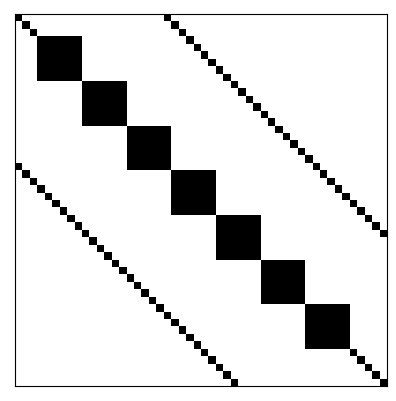
\includegraphics[width=0.45\textwidth]{./cap_sislin/dados/matriz_esparsa_estruturada/main}
  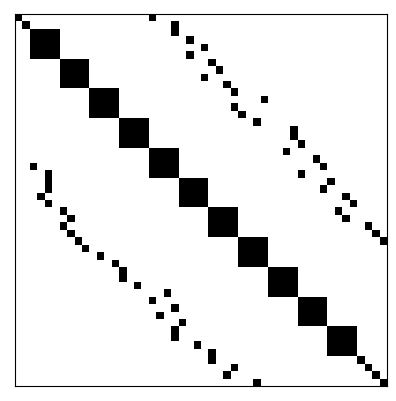
\includegraphics[width=0.45\textwidth]{./cap_sislin/dados/matriz_esparsa_nao_estruturada/main}
  \caption{Esquerda: exemplo de uma matriz esparsa estruturada. Direita: exemplo de uma matriz esparsa não-estruturada.}
  \label{fig:ex_matriz_esparsa_estrutura}
\end{figure}

Matrizes esparsas podem ser classificadas como \emph{estruturadas} ou \emph{não-estruturadas}. Uma matriz estruturada é aquela em que as entradas não-nulas formam um padrão regular. Por exemplo, estão dispostas em poucas diagonais ou formam blocos (submatrizes densas) ao longo de sua diagonal principal. No caso de não haver um padrão regular das entradas não-nulas, a matriz esparsa é dita ser não-estruturada. Consulte a Figura \ref{fig:ex_matriz_esparsa_estrutura} para exemplos.

A \emph{esparsidade} de uma matriz é a porcentagem de elementos nulos que ela tem, i.e. para uma matriz quadrada $n\times n$ tem-se que a esparsidade é
\begin{equation}
  \frac{n_{\text{nulos}}}{n^2}\times 100\%
\end{equation}
Por exemplo, a matriz identidade de tamanho $n=100$ tem esparsidade
\begin{equation}
  \frac{100}{100^2}\times 100\% = 1\% 
\end{equation}

\subsection{Sistemas Tridiagonais}

Um sistema tridiagonal tem a seguinte forma matricial
\begin{equation}\label{eq:sistridiag}
  \begin{bmatrix}
    b_1 & c_1 & & & 0\\
    a_2 & b_2 & c_2 & & \\
    & a_3 & b_3 & \ddots & \\
    & & \ddots & \ddots & c_{n-1}\\
    0 & & & a_n & b_n
  \end{bmatrix}
  \begin{bmatrix}
    x_1\\
    x_2\\
    x_3\\
    \vdots\\
    x_n
  \end{bmatrix} =
    \begin{bmatrix}
    d_1\\
    d_2\\
    d_3\\
    \vdots\\
    d_n
  \end{bmatrix}
\end{equation}
com, $a_1=0$ e $c_n=0$. Ou seja, é um sistema cuja a matriz dos coeficientes é tridiagonal.

Uma \emph{matriz tridiagonal} é uma matriz esparsa estruturada. Mais especificamente, é chamada de \href{https://pt.wikipedia.org/wiki/Matriz_banda}{matriz banda}, em que os elementos não nulos estão apenas em algumas de suas diagonais. Para armazenarmos tal matriz precisamos alocar apenas os seguintes três vetores
\begin{gather}
  a = (0,a_2,\dotsc,a_n)\\
  b = (b_1,b_2,\dotsc,b_n)\\
  c = (c_1,c_2,\dotsc,c_{n-1},0)
\end{gather}
Ou seja, precisamos armazenar $3n$ pontos flutuantes em vez de $n^2$, como seria o caso se a matriz dos coeficientes fosse densa.

\subsubsection{Algoritmo de Thomas}

O Algoritmo de Thomas\footnote{Llewellyn Hilleth Thomas, 1903 - 1992, físico e matemático aplicado britânico. Fonte: \href{https://en.wikipedia.org/wiki/Llewellyn_Thomas}{Wikipedia}.} é uma forma otimizada do Método de Eliminação Gaussiana aplicada à sistemas tridiagonais. Enquanto este requer $O(n^3)$ operações, esse demanda apenas $O(n)$.

Eliminando os termos abaixo da diagonal em \eqref{eq:sistridiag}, obtemos o sistema equivalente
\begin{equation}
  \begin{bmatrix}
    \tilde{b}_1 & c_1 & & & 0\\
      & \tilde{b}_2 & c_2 & & \\
    &  & \tilde{b}_3 & \ddots & \\
    & & \ddots & \ddots & c_{n-1}\\
    0 & & &  & \tilde{b}_n
  \end{bmatrix}
  \begin{bmatrix}
    x_1\\
    x_2\\
    x_3\\
    \vdots\\
    x_n
  \end{bmatrix} =
    \begin{bmatrix}
    \tilde{d}_1\\
    \tilde{d}_2\\
    \tilde{d}_3\\
    \vdots\\
    \tilde{d}_n
  \end{bmatrix}
\end{equation}
Este é obtido pela seguinte iteração
\begin{gather}
  w := \frac{a_i}{b_{i-1}}\\
  b_i := b_i - w c_{i-1}\\
  d_i := d_i - w d_{i-1}
\end{gather}
onde, o $\tilde{}$ foi esquecido de propósito, indicando a reutilização dos vetores $b$ e $d$. A solução do sistema é, então, obtida de baixo para cima, i.e.
\begin{gather}
  x_n = \frac{d_n}{b_n}\\
  x_i = \frac{d_i - c_ix_{i+1}}{b_i},
\end{gather}
com $i=n-1,n-2,\dotsc,1$.

\lstinputlisting[caption=Algoritmo de Thomas]{./cap_sislin/dados/pyTDMA/main.py}

\begin{exer}\label{exer:sislin_tridiag}
  Considere o seguinte sistema linear
  \begin{gather}
    2x_1 - x_2 = 0\\
    x_{i-1} - 3x_i + 4x_{i+1} = \sen\left(i\frac{\pi}{2(n-1)}\right)\\
    x_{n-1} + x_n = 1
  \end{gather}
  \begin{enumerate}[a)]
  \item Compute sua solução usando o Algoritmo de Thomas para $n=3$.
  \item Compare a solução obtida no item anterior com a gerada pela função \href{https://docs.scipy.org/doc/scipy/reference/generated/scipy.linalg.solve.html}{\lstinline+scipy.linalg.solve+}.
  \item Compare a solução com a obtida no item anterior com a gerada pela função \href{https://docs.scipy.org/doc/scipy/reference/generated/scipy.linalg.solve_banded.html}{\lstinline+scipy.linalg.solve_banded+}.
  \item Use o módulo {\python} \href{https://docs.python.org/3/library/timeit.html}{timeit} para comprar a demanda de tempo computacional de cada um dos métodos acima. Compute para $n=10,100,1000,10000$.
  \end{enumerate}
\end{exer}

\begin{exer}
  Considere que o problema de valor de contorno (PVC)
  \begin{gather}
    -u'' = \sen \pi x,\quad 0 < x < 1,\\
    u(0) = 0,\\
    u(1) = 0
  \end{gather}
  seja simulado com o Método das Diferenças Finitas\footnote{Consulte mais em \href{https://phkonzen.github.io/notas/MatematicaNumerica/cap_pvc_sec_mdf.html}{Notas de Aula: Matemática Numérica}.}. Vamos assumir uma discretização espacial uniforme com $n$ nodos e tamanho de malha
  \begin{equation}
    h = \frac{1}{n-1}.
  \end{equation}
  Com isso, temos os nodos $x_i = (i-1)h$, $i=1,2,\dotsc,n$. Nos nodos internos, aplicamos a fórmula de diferenças central
  \begin{equation}
    u''(x_i) \approx \frac{u_{i-1} - 2u_i + u_{i+1}}{h^2},
  \end{equation}
  onde, $u_i \approx u(x_i)$. Com isso, a discretização da EDO fornece
  \begin{equation}
    -\frac{1}{h^2}u_{i-1} + \frac{2}{h^2}u_i - \frac{1}{h^2}u_{i+1} = \sen \pi x_i
  \end{equation}
  para $i=2,3,\dotsc,n-1$. Das condições de contorno temos $u_1 = u_n = 0$. Logo, o problema discreto lê-se: encontrar $u = (u_1,u_2,\dotsc,u_n)\in \mathbb{R}^n$ tal que
  \begin{gather}
    u_1 = 0\\
    -\frac{1}{h^2}u_{i-1} + \frac{2}{h^2}u_i - \frac{1}{h^2}u_{i+1} = \sen \pi x_i\\
    u_n = 0
  \end{gather}
  \begin{enumerate}[a)]
  \item Calcule a solução analítica do PVC.
  \item Use a função \href{https://docs.scipy.org/doc/scipy/reference/generated/scipy.linalg.solve_banded.html}{\lstinline+scipy.linalg.solve_banded+} para computar a solução do problema discreto associado para diferentes tamanhos de malha $h = 10^{-1}, 10^{-2}, 10^{-3}, 10^{-4}$. Compute o erro da solução discreta em relação à solução analítica.
  \item Compare a demanda de tempo computacional se a função \href{https://docs.scipy.org/doc/scipy/reference/generated/scipy.linalg.solve.html}{\lstinline+scipy.linalg.solve+} for empregada na computação da solução discreta.
  \end{enumerate}
\end{exer}

\subsection{Matrizes Banda}

Uma matriz banda é aquela em que os elementos não nulos estão dispostos em apenas algumas de suas diagonais. Consulte a Figura \ref{fig:MatrizBanda}.

\begin{figure}[H]
  \centering
  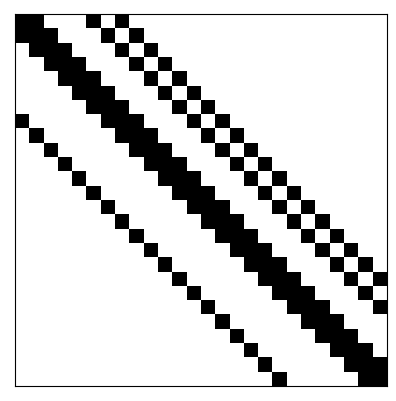
\includegraphics[width=0.45\textwidth]{./cap_sislin/dados/figMatrizBanda/main}
  \caption{Exemplo de uma matriz banda.}
  \label{fig:MatrizBanda}
\end{figure}

\begin{exer}
  Considere o seguinte problema de Poisson\footnote{Baron Siméon Denis Poisson, 1781 - 1840, matemático, engenheiro e físico francês. Fonte: \href{https://en.wikipedia.org/wiki/Sim\%C3\%A9on_Denis_Poisson}{Wikipedia}.}
  \begin{gather}
    u_{xx} + u_{yy} = -\sen(x)\sen(y),~(x, y)\in (0, \pi)\times (0, \pi),\\
    u(0, y) = 0,~y\in [0, \pi],\\
    u(\pi, y) = 0,~y\in [0, \pi],\\
    u(x, 0) = 0,~x\in [0, \pi],\\
    u(x, \pi) = 0,~x\in [0, \pi].
  \end{gather}
  Vamos empregar o Método de Diferenças Finitas para computar uma aproximação para a sua solução. Começamos assumindo uma malha uniforme de $n^2$ nodos
  \begin{gather}
    x_i = (i-1)h\\
    y_j = (j-1)h
  \end{gather}
  com tamanho de malha $h = \pi/(n-1)$, $i=1,2,\dotsc,n$ e $j=1,2,\dotsc,n$. Empregando a Fórmula de Diferenças Central\footnote{Consulte mais em \href{https://phkonzen.github.io/notas/MatematicaNumerica/cap_edp_sec_Poisson.html}{Notas de Aula: Matemática Numérica}.} encontramos o seguinte problema discreto associado
  \begin{gather}
    u_{i, 1} = u_{1, j} = 0,\\
    ~\nonumber\\
    \frac{1}{h^2}u_{i,j-1} + \frac{1}{h^2}u_{i-1,j} - \frac{4}{h^2}u_{i,j} \nonumber\\
    + \frac{1}{h^2}u_{i,j+1} + \frac{1}{h^2}u_{i+1,j} = -\sen(x_i)\sen(y_i),\\
    ~\nonumber\\
    u_{i,n} = u_{n,j} = 0
  \end{gather}
  \begin{enumerate}[a)]
  \item Use a função \href{https://docs.scipy.org/doc/scipy/reference/generated/scipy.linalg.solve_banded.html}{\lstinline+scipy.linalg.solve_banded+} para computar a solução do problema discreto associado para diferentes tamanhos de malha $h = 10^{-1}, 10^{-2}, 10^{-3}, 10^{-4}$. Compute o erro da solução discreta em relação à solução analítica. Compare as aproximações com a solução analítica
    \begin{equation}
      u(x,y) = \frac{1}{2}\sen(x)\sen(y).
    \end{equation}
  \item Compare a demanda de tempo e memória computacional se a função \href{https://docs.scipy.org/doc/scipy/reference/generated/scipy.linalg.solve.html}{\lstinline+scipy.linalg.solve+} for empregada na computação da solução discreta.
  \end{enumerate}
\end{exer}


\subsubsection{Matrizes bloco}

\begin{exer}
  Seja o seguinte PVC
  \begin{gather}
    -u'' + v(x) = f(x),\quad 0<x<1\\
    -v'' - u(x) = g(x),\quad 0<x<1\\
    ~\nonumber\\
    u(0)=u(1)=0\\
    v(0)=v(1)=0
  \end{gather}
  Vamos considerar sua formulação discreta pelo Método de Diferenças Finitas em uma malha uniforme
  \begin{equation}
    x_i = (i-1)h,
  \end{equation}
  com $i=1,2,\dotsc,n$, com tamanho de malha $h = 1/(n-1)$. Usando a fórmula de diferenças central de ordem 2 nas EDOs, obtemos
  \begin{gather}
    -\left(\frac{u_{i-1}-2u_i+u_{i+1}}{h^2}\right) + v_i = f_i\\
    -\left(\frac{v_{i-1}-2v_i+v_{i+1}}{h^2}\right) - u_i = g_i,
  \end{gather}
  sendo, $u_i \approx u(x_i)$, $v_i\approx v(x_i)$, $f_i=f(x_i)$, $g_i = g(x_i)$ com $i=2,\dotsc,n-1$. Considerando as condições iniciais, tomamos $u_1=u_n=v_1=v_n=0$ e multiplicando por $h^2$, temos
  \begin{gather}
    2u_2 - u_3 + h^2v_2 = h^2f_2\\
    -u_{i-1} + 2u_i -u_{i+1} + h^2v_i = h^2f_i\\
    -u_{n-2} + 2u_{n-1} + h^2v_{n-1} = h^2f_{n-1}\\
    ~\nonumber\\
    2v_2 - v_3 - u_2 = h^2g_2\\
    - v_{i-1} + 2v_i -v_{i-1} - h^2u_i = h^2g_i\\
    - v_{n-2} + 2v_{n-1}  - h^2u_{n-1} = h^2g_{n-1}\\    
  \end{gather}
  onde, $i=3,\dotsc,n-2$.

  As equações acima formam um sistema linear $2(n-2)\times 2(n-2)$. Podemos escrever sua forma matricial
  \begin{equation}
    Aw = h
  \end{equation}
  de várias formas a depender da escolha do vetor $w$ em função de $u$ e $v$. Vamos aqui considerar duas delas:
  \begin{itemize}
  \item[F1.] $w = (u_2,v_2,\dotsc,u_{n-1},v_{n-1})$
    \begin{gather}
      u_i = w_{2(i-1)-1}\\
      f_i = h_{2(i-1)-1}\\
      ~\nonumber\\
      v_i = w_{2(i-1)}\\
      g_i = h_{2(i-1)}
    \end{gather}
  \item[F2.] $w = (u_2,\dotsc,u_{n-1},v_2,\dotsc,v_{n-1})$
    \begin{gather}
      u_i = w_{i-1}\\
      f_i = h_{i-1}\\
      ~\nonumber\\
      v_i = w_{i+n-3}\\
      g_i = h_{i+n-3}
    \end{gather}    
  \end{itemize}
\end{exer}
